\subsection*{IMPORTANT: A difference between regression and classification}

    Here is an important misconception that comes up between regression and classification.
    
    Both functions use the equation
    
    \begin{equation}
        \theta^T x + \theta_0
    \end{equation}
    
    So, one might think of them as interchangeable.
    
    However, they are \redd{not}. Why is that?
    
    \begin{figure}[H]

        
        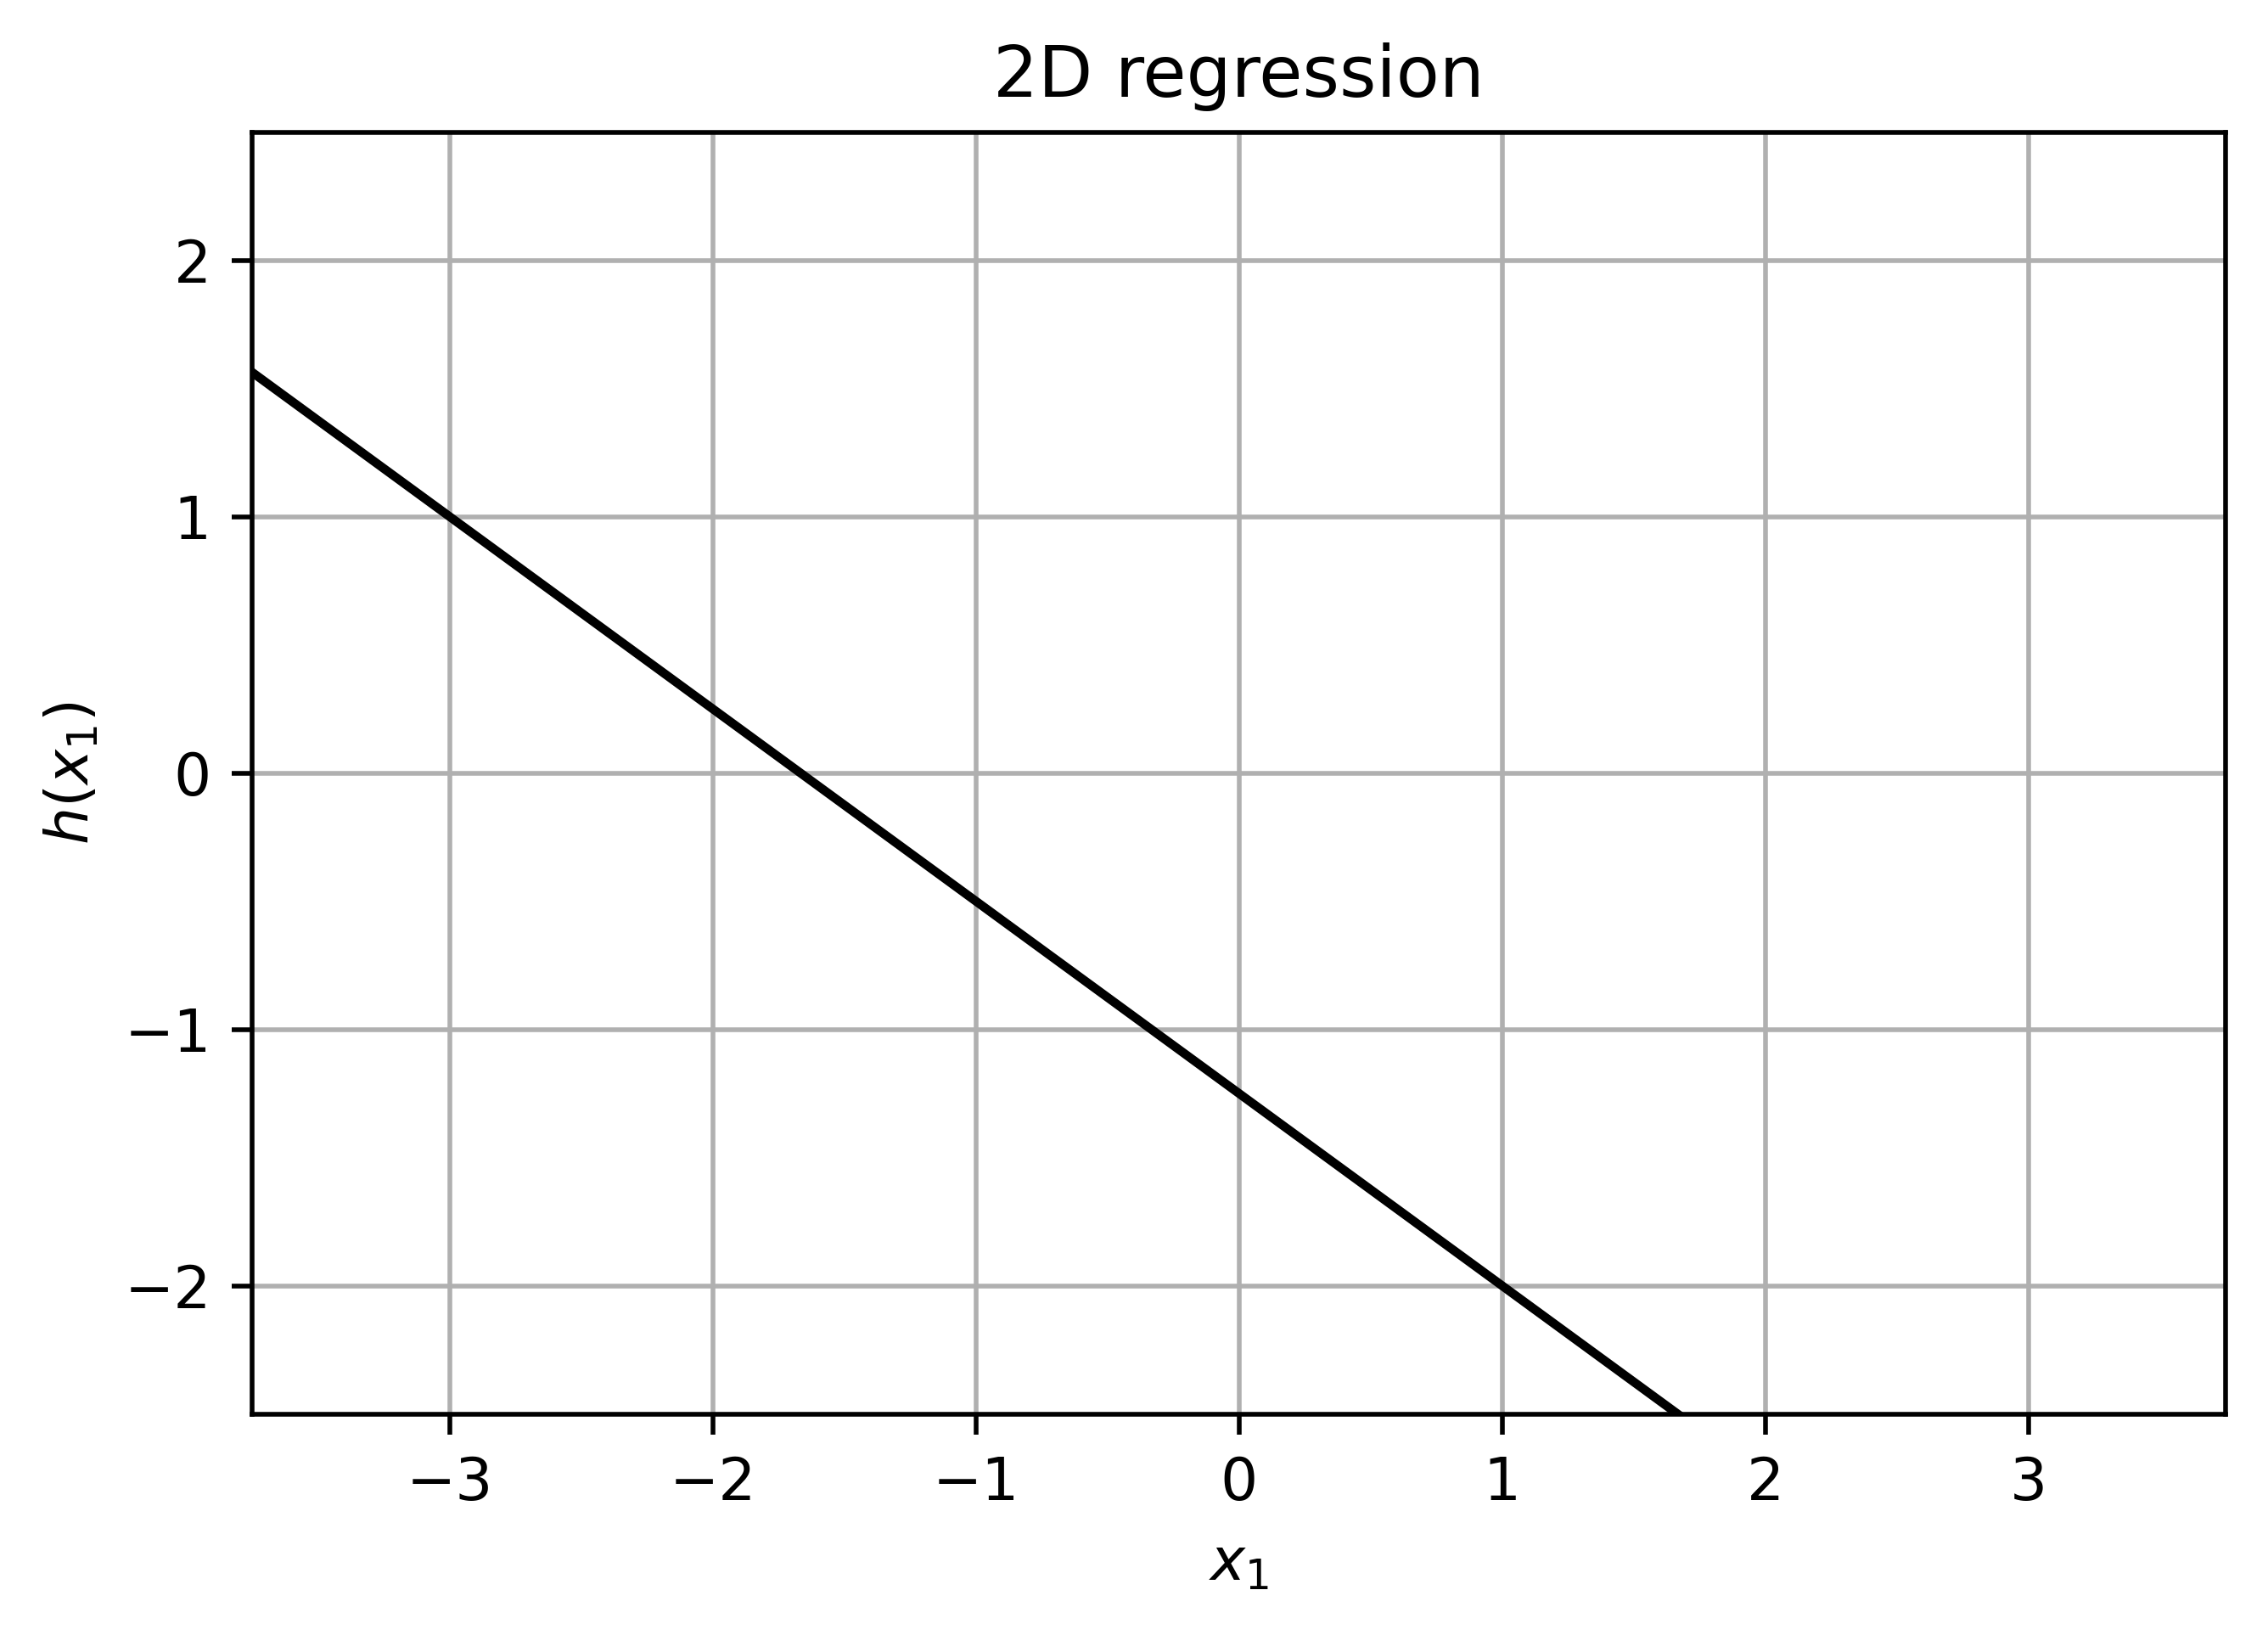
\includegraphics[width=70mm,scale=0.5]{images/classification_images/2d_regression_versus.png}
        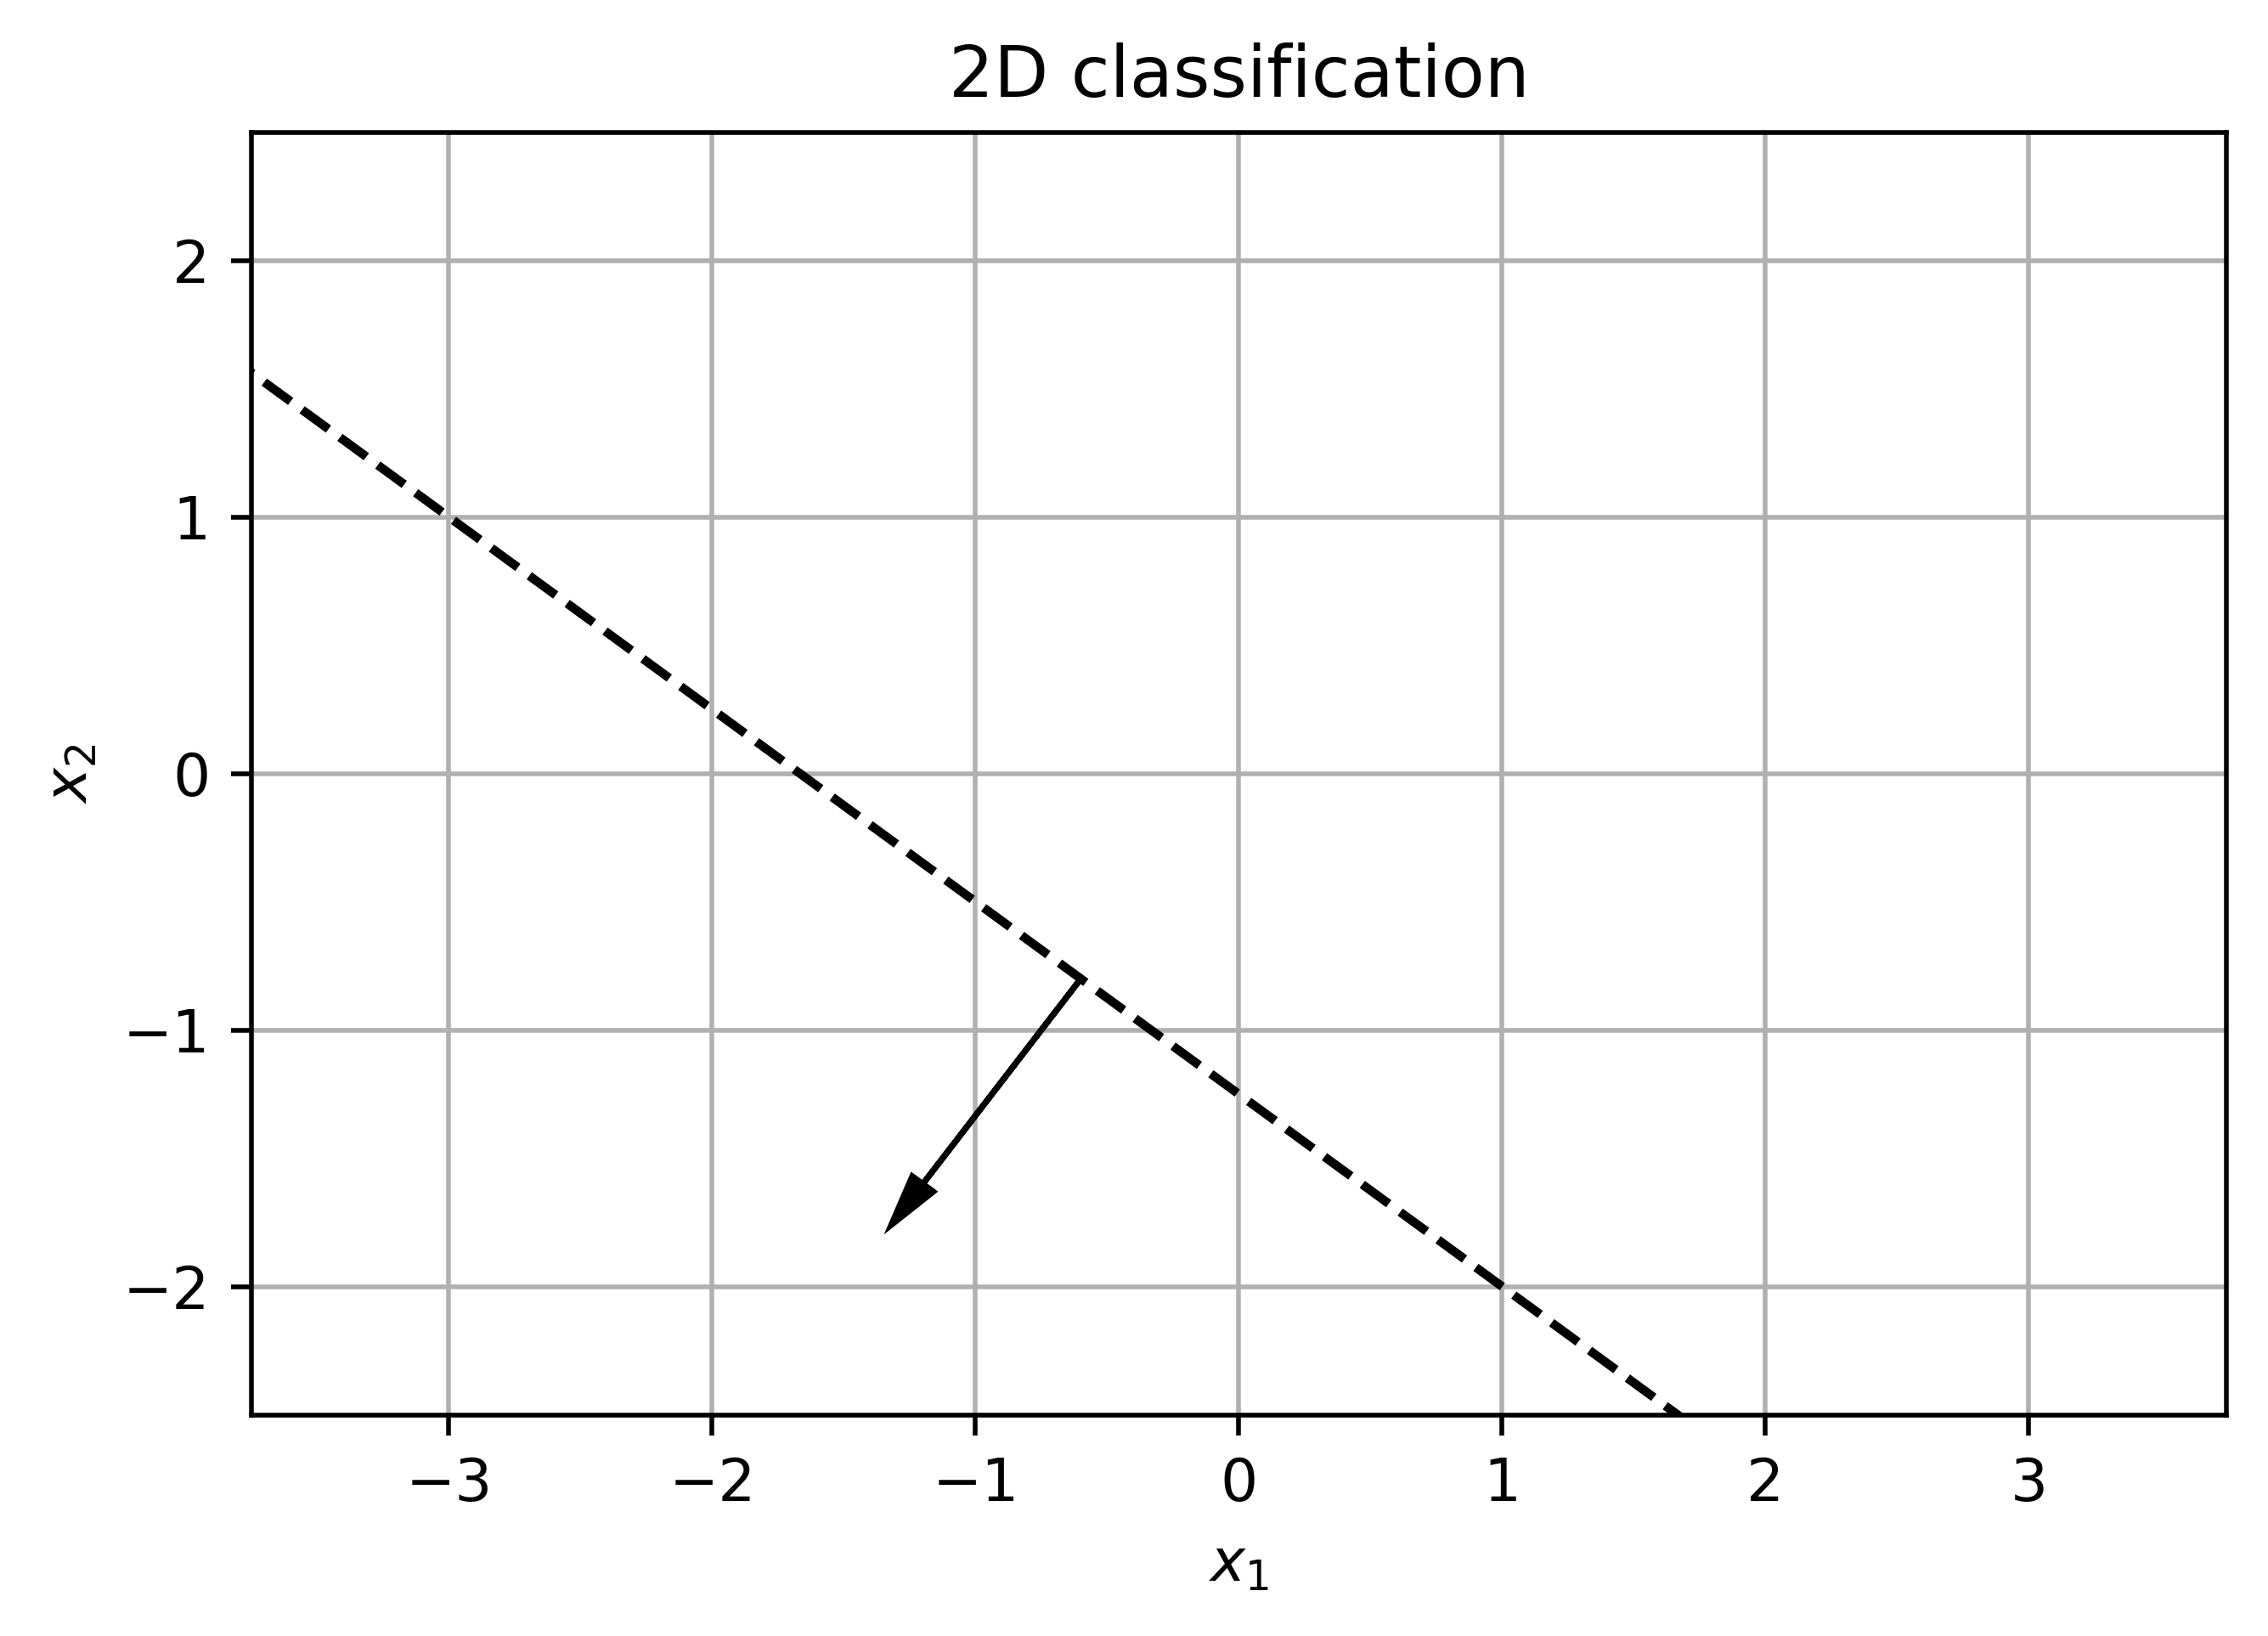
\includegraphics[width=70mm,scale=0.5]{images/classification_images/2d_classification_versus.png}

        \caption*{These two plots look almost the same, but represent completely different things!}
    \end{figure}
    
    Notice that these two plots are \textbf{both} plotted in 2-D, and both have a \textbf{line} plotted. But, they \textbf{aren't} as \textbf{similar} as they look. 
    
    Notice, for example, that the regression plot has \textbf{only} $x_1$, while the classification plot has $x_1$ \textbf{and} $x_2$.
    
    The reason why? The \textbf{output}.
    
    \begin{itemize}
        \item In \vocab{regression}, the output is a \textbf{real number}: every point on that line represents an input $x_1$, and an output $h(x_1)$.
            
            \begin{itemize}
                \item This plot can only contain \textbf{one} input variable: the \textbf{second} axis is reserved for the \textbf{output}!
            \end{itemize}
        
        \item In \vocab{classification}, the output is \textbf{binary}. So, that line represents only the \textbf{values} where the output is $h(x)=0$. 
            \begin{itemize}
                \item This plot can contain \textbf{two} input variables: $x_1$ and $x_2$. Rather than \textbf{displaying} the output, we only show one \textbf{slice} of the output: the $h(x)=0$ slice.
            \end{itemize}
    \end{itemize}
    
    If we think in terms of $f(x) = \theta^Tx +\theta_0$, we can compare them directly.
    
    The regression plot shows the exact value on the y-axis. If we want to know what $f(x_1=1)$ looks like, we can check the plot: we just get $f(1)=-2$.
    
    \begin{figure}[H]
        \centering
        
        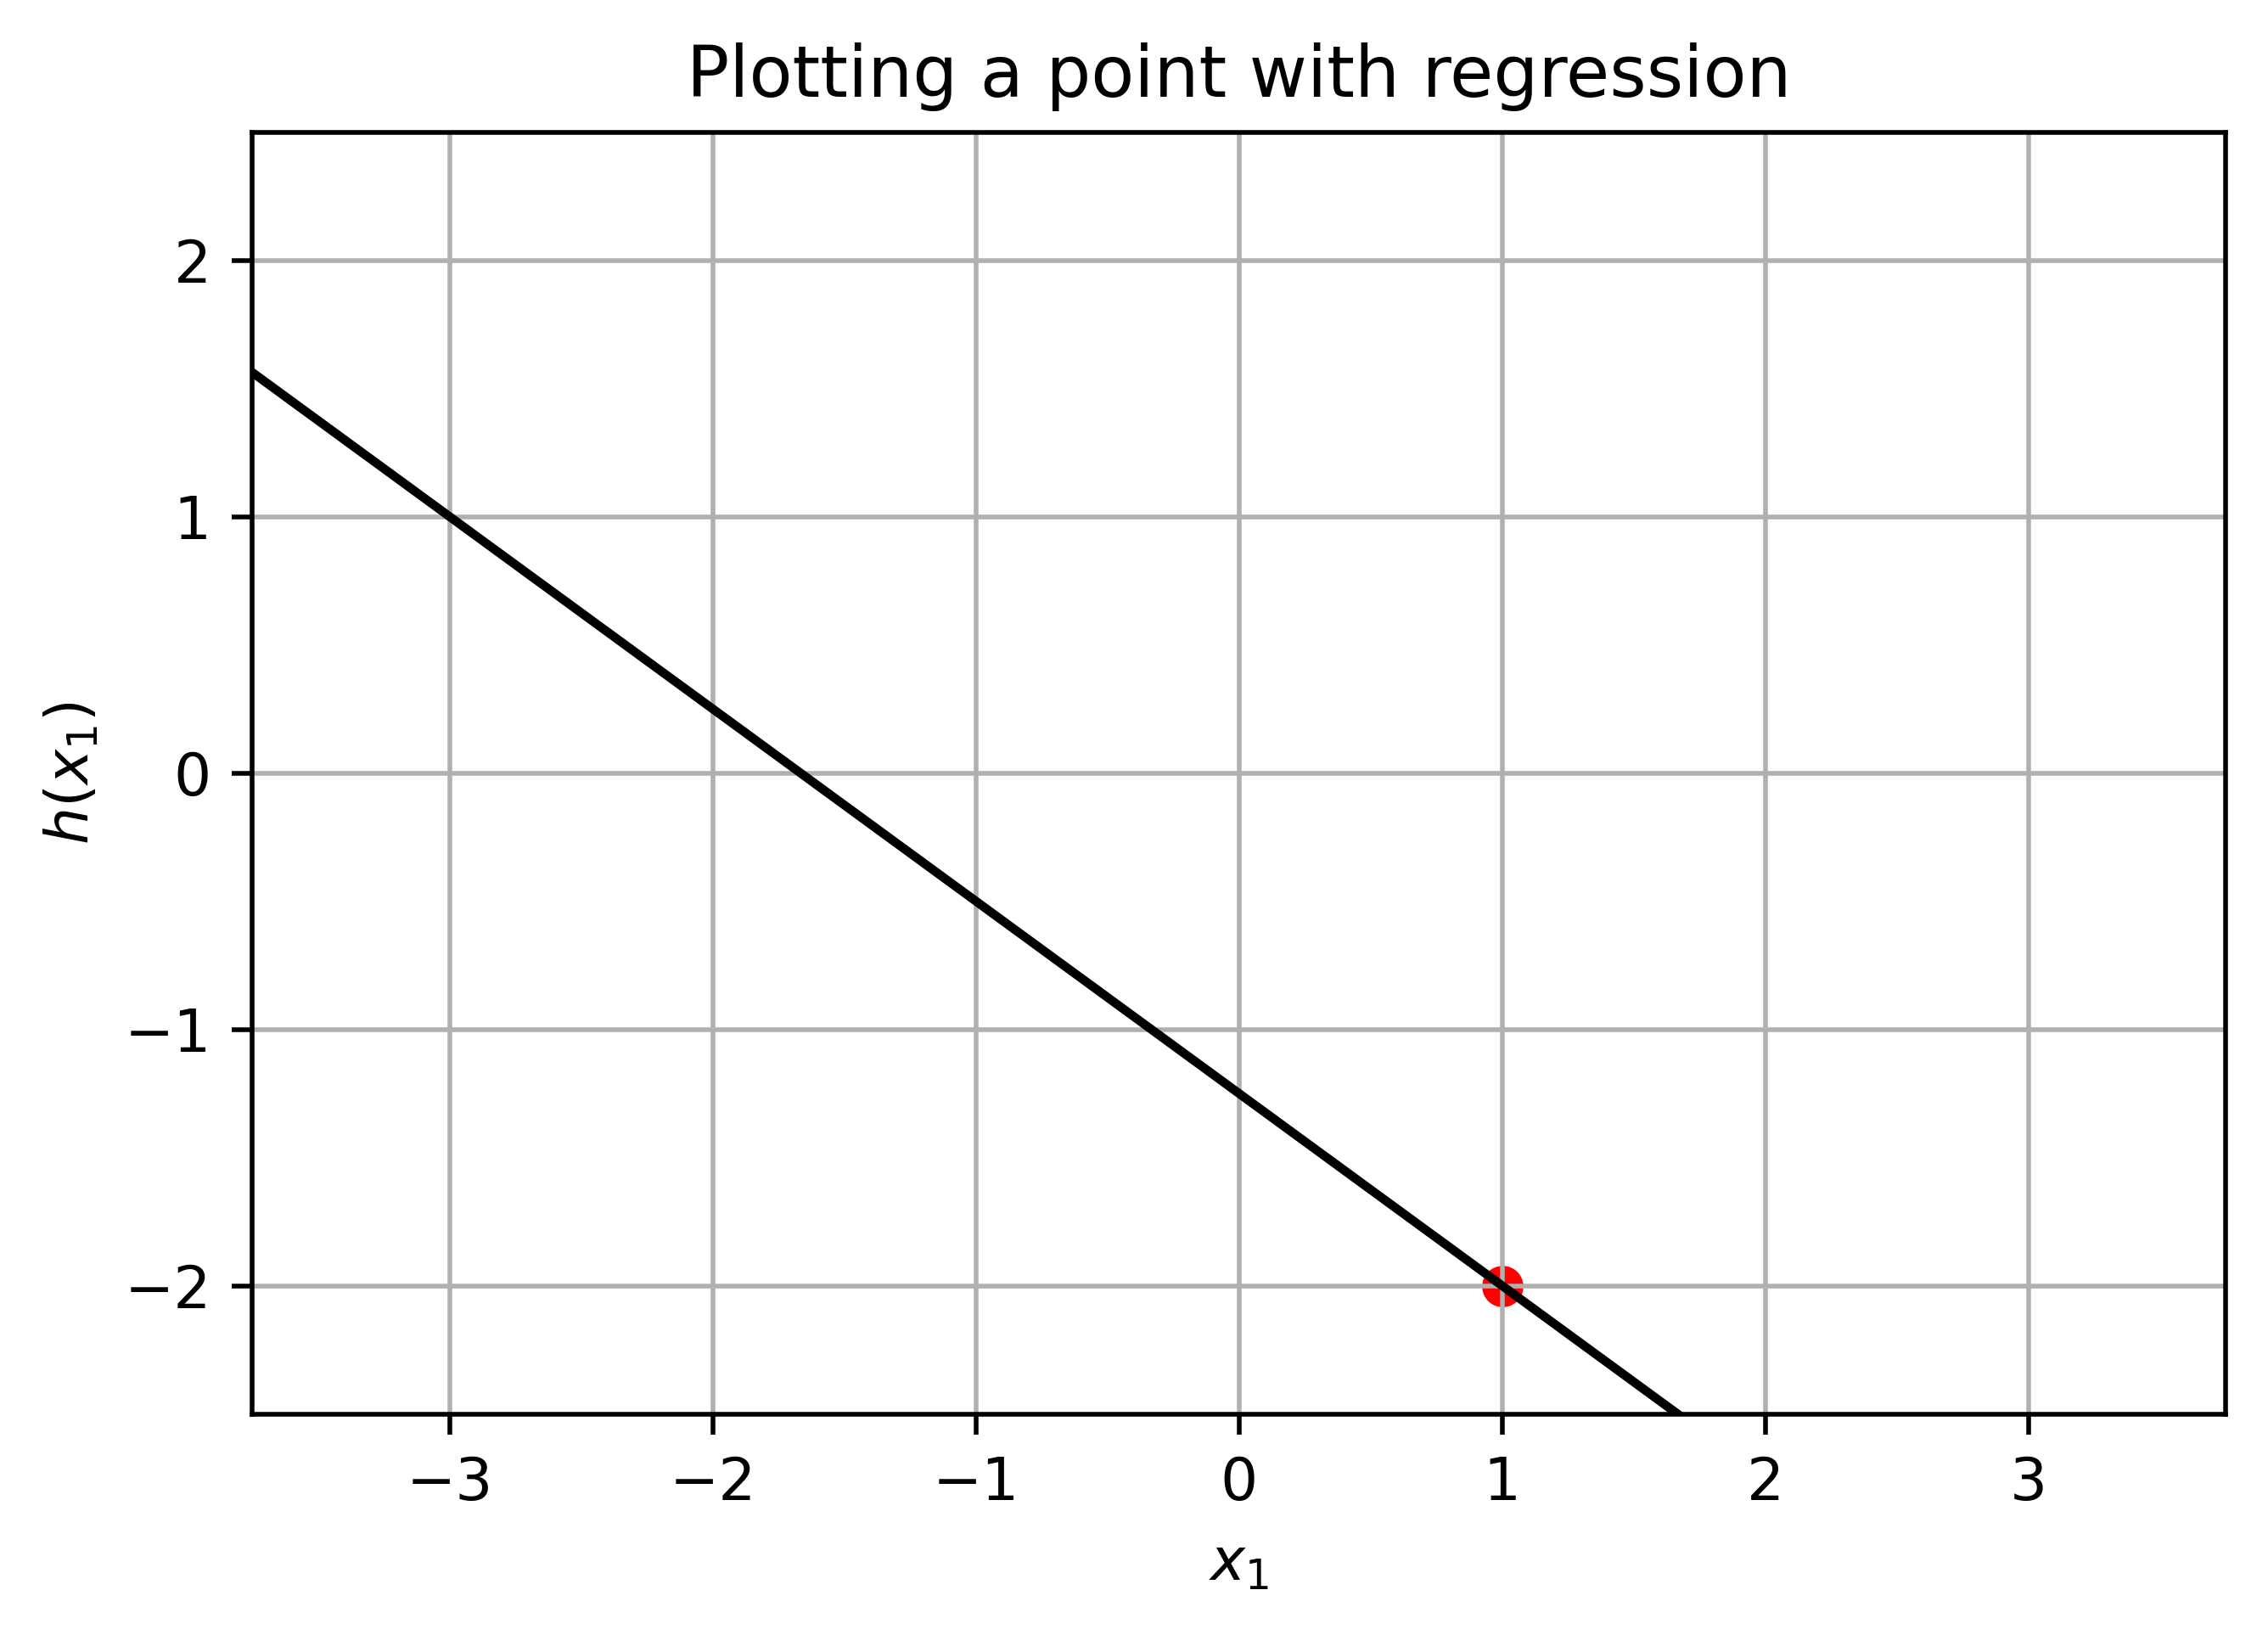
\includegraphics[width=70mm,scale=0.5]{images/classification_images/2d_regression_plot.png}
        \caption*{We have one input, and we get the exact value of our output.}
    \end{figure}
    
    But the classification plot \textbf{doesn't}! We aren't given the value of $\theta^Tx +\theta_0$ at $x=(1,0)$: we just know that it's \textbf{negative}.
    
    \begin{figure}[H]
        \centering
        
        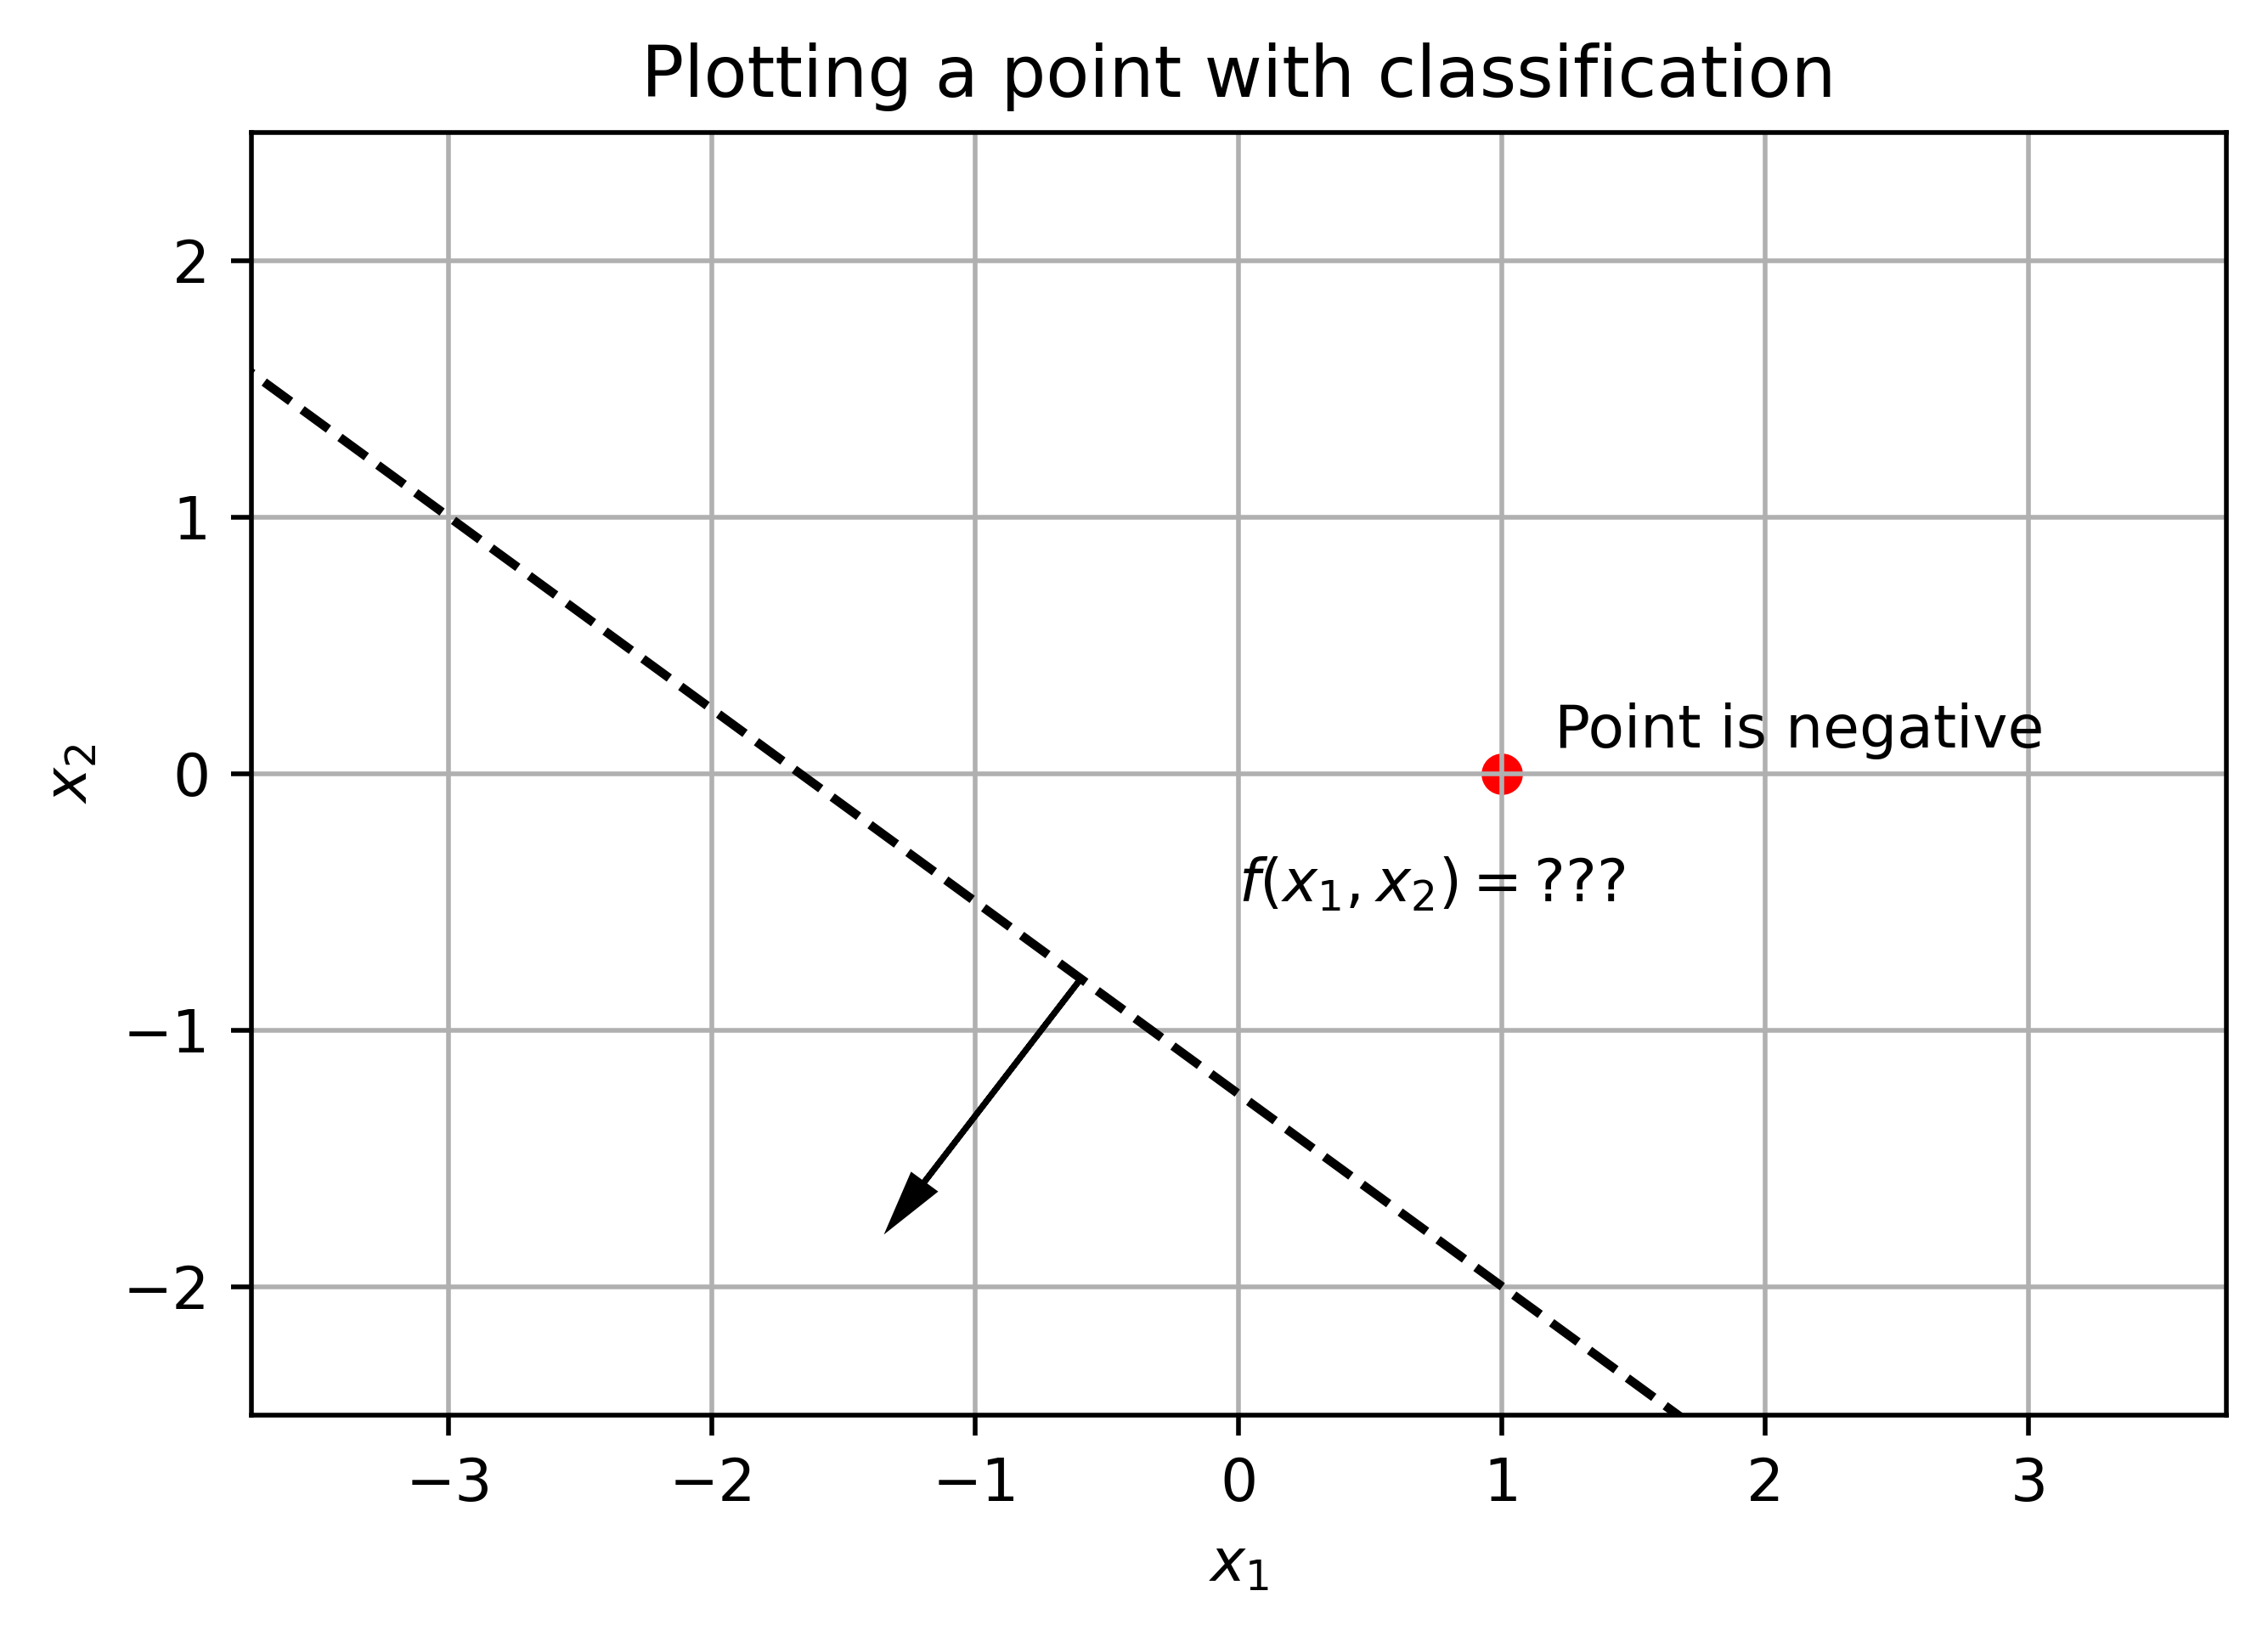
\includegraphics[width=70mm,scale=0.5]{images/classification_images/2d_classification_plot.png}
        \caption*{We have two input, and we \textbf{don't} get the exact output.}
    \end{figure}
    
    If we wanted to know the exact value of our 2-D classification, we would need to view it as a plane in 3-D space.
    
    This is the trade-off between these two plots: one gives more information about the output, and the other allows for more inputs in a lower dimension.\\
    
    \begin{clarification}
        \vocab{Regression} and \vocab{classification} plots that look the same, have \vocab{different functions}: 
        
        When looking at the output of $f(x)=\theta^T x + \theta_0$,
        \begin{itemize}
            \item A \purp{regression} plot gives the \gren{exact numeric} $f(x)$.
            
            \item A \purp{classification} plot only gives the \gren{sign} of the $f(x)$.
        \end{itemize}
        
        When plotting $n$ inputs,
            \begin{itemize}
                \item A \purp{regression} plot uses a $d+1$ dimensions ($d$-dim hyperplane) to plot: +1 for the \gren{output}.
                \item A \purp{classification} plot only needs $d$ dimensions ($(d-1)$-dim hyperplane): we only see the $f(x)=0$ \gren{hyperplane}.
            \end{itemize}
    \end{clarification}
    
    Why do we need $d+1$ dimensions to plot a $d$-dimensional \textbf{hyperplane}? You can think of it this way: a \textbf{line} in 2-D space is a 1-D \textbf{hyperplane}: we have only \textbf{one axis} we can move on the line.
        
    \begin{figure}[H]
        \centering
        
        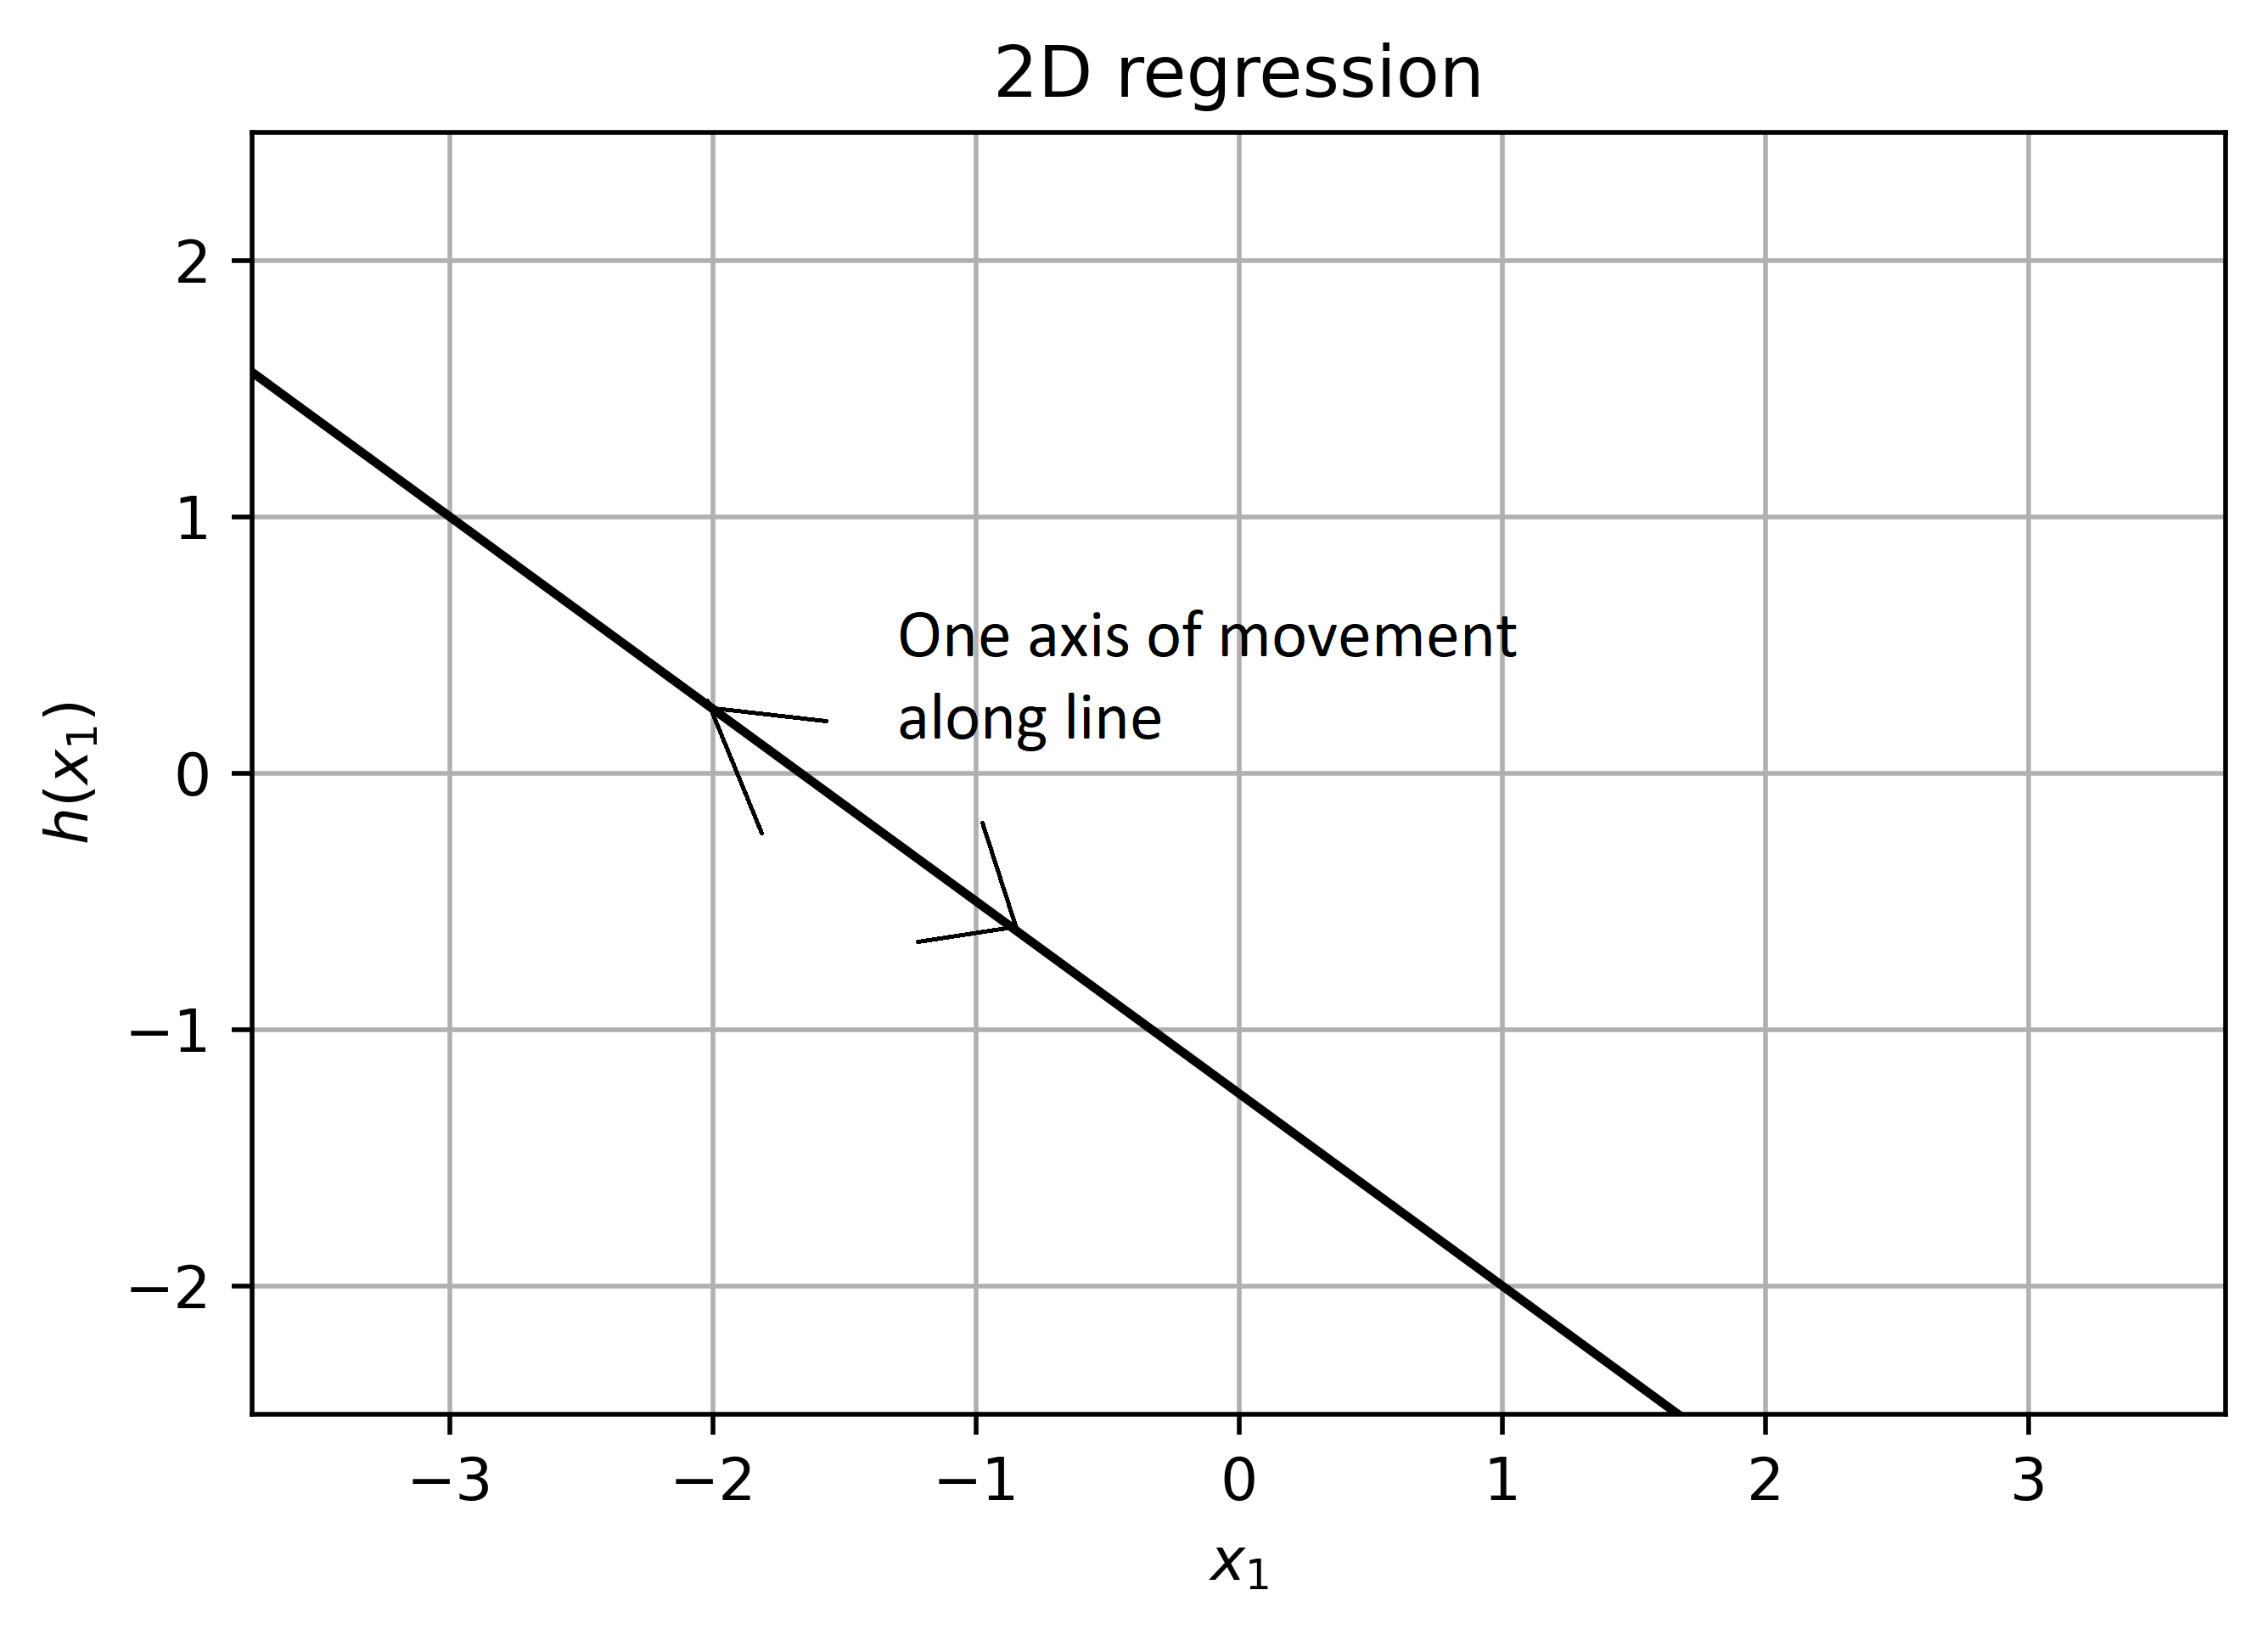
\includegraphics[width=70mm,scale=0.5]{images/classification_images/2d_regression_1d_hyperplane.png}
        \caption*{Our plot is 2-D, but we can only move along one axis on our line!}
    \end{figure}    
    
    Because of these differences, $\theta$ also acts differently:\\
    
    \begin{clarification}
        $\theta$ appears differently in 2-D regression and classification:
        
        \begin{itemize}
            \item In \vocab{2-D regression}, $\theta$ is the \purp{slope} of the line
            
                \begin{equation}
                    h(x) = \theta x + \theta_0
                \end{equation}
            
            \item In \vocab{2-D classification}, $\theta$ is the \purp{normal vector} of the line
            
                \begin{equation}
                    0 = \theta^T x + \theta_0
                \end{equation}
            
        \end{itemize}
    \end{clarification}